\documentclass{standalone}
\usepackage[utf8]{inputenc}
\usepackage{tikz}
\usetikzlibrary{shapes.geometric, arrows, positioning, fit, backgrounds, calc, matrix}
\usepackage{helvet}
\renewcommand{\familydefault}{\sfdefault}

% Colors are still useful in preamble for standalone, but we'll use literal colors or re-define them if needed in main.
% To be safe, we use standard colors in the styles below or define them in the tikzpicture scope if they are custom.
% Defining them globally in the doc body is safest for input.

\definecolor{frozen}{RGB}{200, 200, 200}
\definecolor{trainable}{RGB}{255, 150, 100}
\definecolor{data}{RGB}{100, 180, 255}
\definecolor{process}{RGB}{220, 220, 250}

\begin{document}
% We embed styles here so they are preserved when imported via \input into main.tex
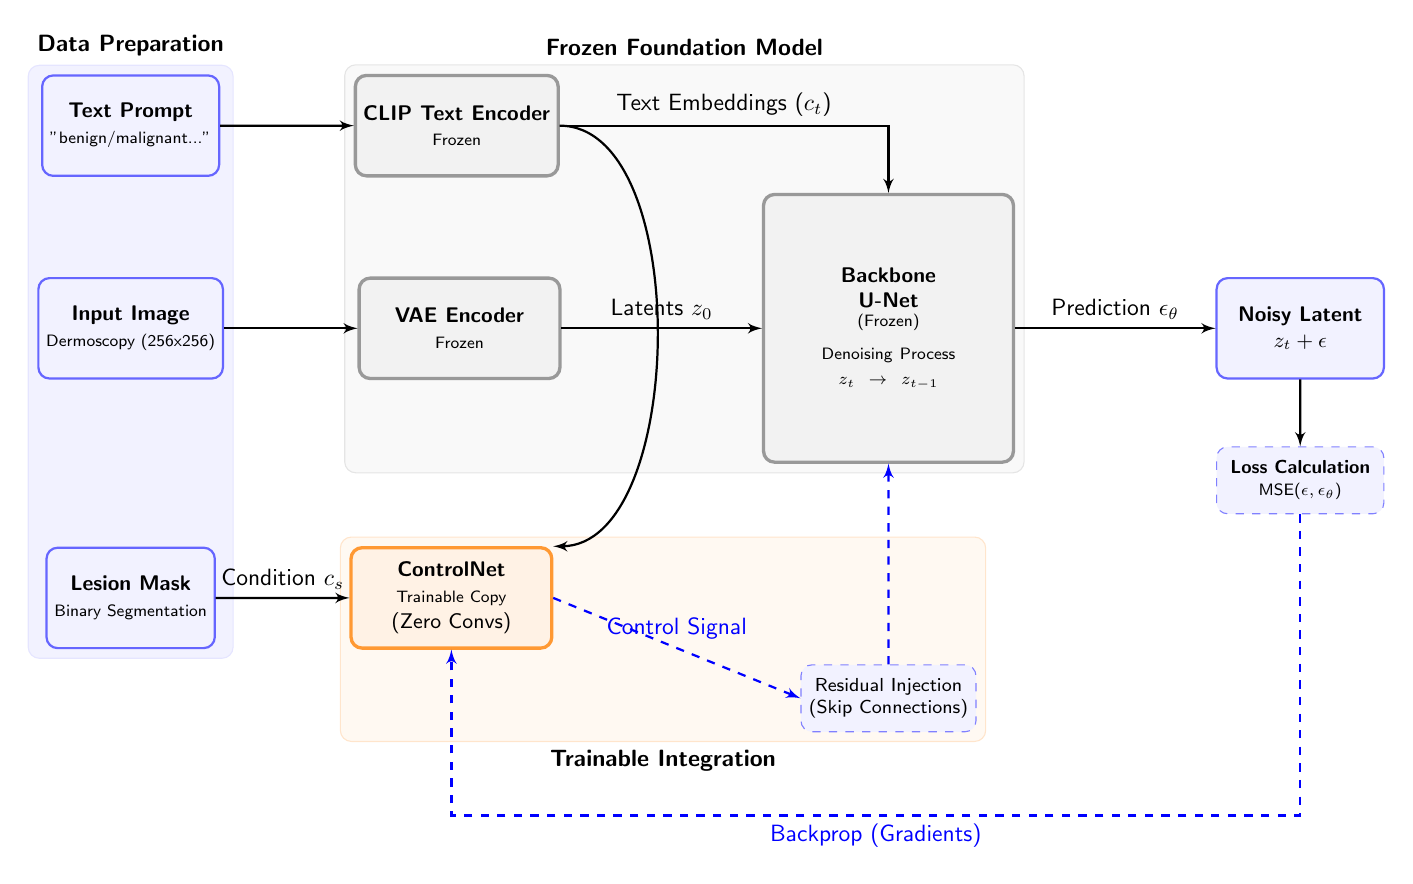
\begin{tikzpicture}[
    node distance=2.5cm, 
    auto, 
    scale=0.85, 
    transform shape, 
    ampersand replacement=\&,
    % Styles embedded for portability
    box_frozen/.style={rectangle, rounded corners, minimum width=3cm, minimum height=1.5cm, align=center, draw=gray!80, fill=gray!10, very thick, font=\sffamily\small},
    box_trainable/.style={rectangle, rounded corners, minimum width=3cm, minimum height=1.5cm, align=center, draw=orange!80, fill=orange!10, very thick, font=\sffamily\small},
    box_data/.style={rectangle, rounded corners, minimum width=2.5cm, minimum height=1.5cm, align=center, draw=blue!60, fill=blue!5, thick, font=\sffamily\small},
    process/.style={rectangle, rounded corners, minimum width=2.5cm, minimum height=1cm, align=center, draw=blue!50, fill=blue!5, dashed, font=\sffamily\footnotesize},
    line/.style={draw, -latex', thick},
    dashedline/.style={draw, -latex', dashed, thick, blue}
]

    % --- LAYER 1: DATA INPUTS (Left Side) ---
    \node [box_data] (img) {\textbf{Input Image}\\\scriptsize Dermoscopy (256x256)};
    \node [box_data, below=2.5cm of img] (mask) {\textbf{Lesion Mask}\\\scriptsize Binary Segmentation};
    \node [box_data, above=1.5cm of img] (prompt) {\textbf{Text Prompt}\\\scriptsize "benign/malignant..."};

    % --- LAYER 2: ENCODERS (Column 2) ---
    \node [box_frozen, right=2cm of img] (vae) {\textbf{VAE Encoder}\\\scriptsize Frozen};
    \node [box_trainable, right=2cm of mask] (controlnet) {\textbf{ControlNet}\\\scriptsize Trainable Copy\\(Zero Convs)};
    \node [box_frozen, right=2cm of prompt] (clip) {\textbf{CLIP Text Encoder}\\\scriptsize Frozen};

    % --- LAYER 3: DIFFUSION PROCESS (Column 3) ---
    % UNet is the core, sits in the middle
    \node [box_frozen, right=3cm of vae, minimum height=4cm, text width=3.5cm] (unet) {\textbf{Backbone}\\\textbf{U-Net}\\\scriptsize (Frozen)\\\vspace{0.2cm}Denoising Process\\$z_t \rightarrow z_{t-1}$};
    
    % Control Signal Injection
    \node [process, below=of unet, yshift=-0.5cm] (injection) {Residual Injection\\(Skip Connections)};

    % --- LAYER 4: OUTPUT & LOSS (Far Right) ---
    \node [box_data, right=3cm of unet] (output) {\textbf{Noisy Latent}\\$z_t + \epsilon$};
    \node [process, below=1cm of output] (loss) {\textbf{Loss Calculation}\\\scriptsize MSE($\epsilon, \epsilon_\theta$)};
    
    % --- CONNECTIONS ---
    
    % Text Flow
    \draw [line] (prompt) -- (clip);
    \draw [line] (clip) -| node[near start, above] {Text Embeddings ($c_t$)} (unet.north);
    \draw [line] (clip.east) .. controls +(2,0) and +(2,0) .. (controlnet.north east);

    % Image Flow
    \draw [line] (img) -- (vae);
    \draw [line] (vae) -- node[above] {Latents $z_0$} (unet);

    % Control Flow
    \draw [line] (mask) -- node[above] {Condition $c_s$} (controlnet);
    % Route through Injection Node
    \draw [dashedline] (controlnet.east) -- node[above] {Control Signal} (injection.west);
    \draw [dashedline] (injection.north) -- (unet.south);
    
    % Training Loop (Symbolic)
    \draw [line] (unet) -- node[above] {Prediction $\epsilon_\theta$} (output);
    \draw [line] (output) -- (loss);
    % Reroute backprop to go under everything
    \draw [dashedline] (loss.south) -- ++(0,-4.5cm) -| node[near start, below] {Backprop (Gradients)} (controlnet.south);

    % --- GROUPING & BACKGROUNDS ---
    \begin{scope}[on background layer]
        % Blue Zone: Data Preparation
        \node [fill=blue!5, fit=(img) (mask) (prompt), rounded corners, draw=blue!10, label=above:\textbf{Data Preparation}] (prep_zone) {};
        
        % Gray Zone: Pretrained Frozen Model
        \node [fill=gray!5, fit=(clip) (vae) (unet), rounded corners, draw=gray!20, label=above:\textbf{Frozen Foundation Model}] (frozen_zone) {};
        
        % Orange Zone: Trainable Parts
        \node [fill=orange!5, fit=(controlnet) (injection), rounded corners, draw=orange!20, label=below:\textbf{Trainable Integration}] (train_zone) {};
    \end{scope}

\end{tikzpicture}
\end{document}
